\documentclass[11pt,letterpaper]{article}

\input{../../../../.config/latex/preamble_v1.tex}
\lightmode

\title{\textbf{Math 55b Problem Set 6}}

\begin{document}
\maketitle

\textit{I collaborated with AJ LaMotta for this problem set.}

\begin{problem}%59.4
    Suppose $X=U\cup V$ where $U,V$ are open subsets of $X$. Suppose that $U\cap V$ is path connected and that $x_0\in U\cap V$. Let $i,j$ be the inclusion mappings of $U$ and $V$ respectively into $X$. Then the images of the induced homomorphisms
    \[
        i_* : \pi_1(U,x_0) \to \pi_1(X,x_0)\quad \mathrm{and}\quad j_* : \pi_1(V,x_0) \to \pi_1(X,x_0)
    \]
    generate $\pi_1(X,x_0)$ by Theorem 59.1.
    \begin{enumerate}[(a)]
        \item What can you say about the fundamental group of $X$ if $j_*$ is the trivial homomorphism? If both $i_*$ and $j_*$ are trivial?
        \item Give an example where $i_*$ and $j_*$ are trivial but neither $U$ nor $V$ have trivial fundamental groups.
    \end{enumerate} 
\end{problem}

\begin{solution}
    \textbf{(a)} If $j_*$ is trivial, then $\pi_1(X,x_0)$ is generated by $i_*(\pi_1(U,x_0))$ so $\pi_1(X,x_0)$ is isomorphic to a quotient of the group $\pi_1(U,x_0)$. If both $i_*$ and $j_*$ are trivial, then $\pi_1(X,x_0)$ is trivial so $x_0$ is in a simply connected path component. 

    \textbf{(b)} Let $X=\R^2$ and define $U=\R^2-\{(1,0)\}$ and $V=\R^2-\{(-1,0)\}$. Clearly $U\cap V$ is path connected. Letting $x_0\in U\cap V$, clearly $\pi_1(U,x_0)\cong \pi_1(V,x_0)\cong \Z$, since $U$ and $V$ have deformation retractions onto circles. Yet $\pi_1(\R^2,x_0)$ is trivial, so the induced homomorphisms $i_*$ and $j_*$ must also be trivial homomorphisms. 
\end{solution}

\begin{problem}%60.5
    Consider the covering map indicated in the figure:
    \medskip
    \begin{center}
        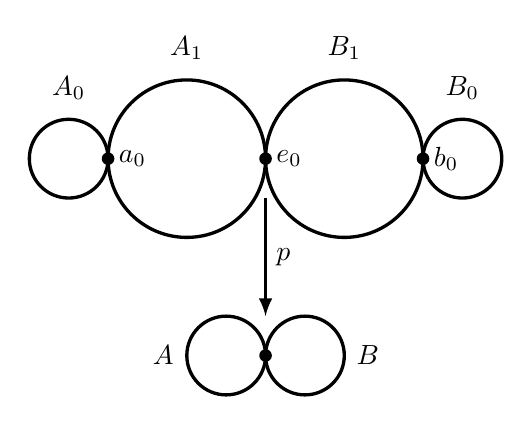
\begin{tikzpicture}
            \begin{scope}[very thick]
                \fill[] (0,0) circle (0.08) node[right] {$e_0$};
                \fill[] (2,0) circle (0.08) node[right] {$b_0$};
                \fill[] (-2,0) circle (0.08) node[right] {$a_0$};
                \node[] at (-1,1.4) {$A_1$};
                \node[] at (1,1.4) {$B_1$};
                
                \draw[] (1,0) circle (1);

                \draw[] (-1,0) circle (1);
                \draw[] (2.5, 0) circle (0.5);
                \draw[] (-2.5, 0) circle (0.5);
                \node[] at (-2.5,0.9) {$A_0$};
                \node[] at (2.5,0.9) {$B_0$};
            \end{scope}
            
            \draw[-latex, very thick] (0,-0.5) -- node[right] {$p$} (0,-2);

            \begin{scope}[very thick, yshift=-2.5cm]
                \fill[] (0,0) circle (0.08);

                \draw[] (0.5,0) circle (0.5);
                \draw[] (-0.5,0) circle (0.5);
                \node[] at (-1.3,0) {$A$};
                \node[] at (1.3,0) {$B$};
            \end{scope}
        \end{tikzpicture}
    \end{center}
    \medskip
    Here $p$ wraps $A_1$ around $A$ twice and wraps $B_1$ around $B$ twice; $p$ maps $A_0$ and $B_0$ homeomorphically onto $A$ and $B$, respectively. Use this covering space to show that the fundamental group of the figure eight is not abelian.
\end{problem}

\begin{solution}
    Similarly to the proof in Munkres, let $\alpha$ be the loop going counterclockwise around $A$ and let $\beta$ be the loop going counterclockwise around $B$. Then lifting $\alpha*\beta$ to a path starting at $e_0$, we get a path going along the bottom of $A_1$ to $a_0$ and then going counterclockwise around $A_0$. Similarly, lifting $\beta*\alpha$ gives a path going along the top of $B_1$ to $b_0$ and then going counterclockwise around $B_0$ back to $b_0$. Since these lifts have different endpoints, $\alpha*\beta\neq \beta*\alpha$ so the fundamental group of the figure eight is not abelian. 
\end{solution}

\begin{problem}%74.1
    Show that if $n>1$, every continuous map $f : S^n \to S^1$ is nullhomotopic. %Use the lifting lemma
\end{problem}

\begin{solution}
    Recall the covering map $p : \R \to S^1$ given by $p(t)=e^{2\pi i t}$. Now assume without loss of generality that $f^{-1}(1)$ is nonempty (otherwise rotate the map), let $x_0\in f^{-1}(1)$. Then $f_*(\pi_1(S^n, x_0))=\{0\}$ since $S^n$ is simply connected for $n>1$. Then by the general lifting lemma, there must be a map $\widetilde{f} : S^n \to \R$ such that $\widetilde{f}(x_0)=0$ and $p\circ\widetilde{f}=f$. We claim that $f\simeq c_{1}$, the constant map which takes every element to $1$. First note that $\widetilde{f} \simeq c_{0}$, since $\R$ is contractible. Let $H : I\times S^n \to \R$ be some homotopy with $H(0,x)=\widetilde{f}(x)$ and $H(1,x)=0$. Then consider $p\circ H : I\times S^n \to S^1$. This is a homotopy with $H(0,x)=p(\widetilde{f}(x))=f(x)$ and $H(1,x)=1$, so $f\simeq c_{1}$ as desired.   
\end{solution}

\begin{problem}%74.4
    Let $T=S^1\times S^1$ be the torus. There is an isomorphism of $\pi_1(T,b_0\times b_0)$ with $\Z\times \Z$ induced by projections of $T$ onto its two factors.
    \begin{enumerate}[(a)]
        \item Find a covering space of $T$ corresponding to the subgroup of $\Z\times \Z$ generated by the element $m\times 0$, where $m$ is a positive integer.
        \item Find a covering space of $T$ corresponding to the trivial subgroup of $\Z\times \Z$.
        \item Find a covering space of $T$ corresponding to the subgroup of $\Z\times \Z$ generated by $m\times 0$ and $n\times 0$ where $m,n$ are positive integers. 
    \end{enumerate} 
\end{problem}

\begin{solution}
    Let $p_n : S^1 \to S^1$ given by $p_n(z) = z^n$ be an $n$-sheeted covering of the circle, and let $q : \R \to S^1$ given by $q(t)=e^{2\pi i t}$ be the universal covering space of the circle. 

    \textbf{(a)} Consider the covering space $p_m\times q : S^1\times \R \to S^1\times S^1=T$. Then by basic properties of the induced homomorphism, $(p_m\times q)_* = (p_m)_* \times q_*$ so $\Ima((p_m\times q)_*)=m\Z\times 0$, which is the desired subgroup of $\Z\times \Z$. 

    \textbf{(b)} This is just the universal cover of $T$, i.e. a simply connected covering space of $T$. Consider the covering space $q\times q : \R^2 \to S^1\times S^1=T$. Since $\R^2$ is simply connected, it clearly corresponds to the trivial subgroup of $\Z\times \Z$.

    \textbf{(c)} Consider the covering space $p_m\times p_n : S^1\times S^1 \to S^1\times S^1=T$. As in (a), we have $\Ima((p_m\times p_n)_*)=\Ima((p_m)_*)\times \Ima((p_n)_*)=m\Z\times n\Z$, which is the desired subgroup of $\Z\times \Z$.
\end{solution}

\begin{problem}
    Show that there do not exist any covering maps:
    \begin{enumerate}[(a)]
        \item from $\RP^2$ to $T$ (torus),
        \item from $T$ to $\RP^2$,
        \item from $\R^2$ to $\RP^2$.
    \end{enumerate}
\end{problem}

\begin{solution}
    In lecture, we proved that $\pi_1(\RP^2)=\Z/2\Z$, $\pi_1(T)=\Z\times \Z$, and $\pi_1(\R^2)=\{0\}$. Furthermore, for any covering map $p : E \to B$, the induced homomorphism $p_* : \pi_1(E,e_0) \to \pi_1(B, p(e_0))$ is an injection. This shows that there is no covering map from $\RP^2$ to $T$ or $T$ to $\RP^2$ to $T$, since there can be no injective homorphism $\Z /2\Z\to \Z\times \Z$ or $\Z\times \Z \to \Z/2\Z$. Now suppose for the sake of contradiction that there were a covering map $p : \R^2 \to \RP^2$, and consider the natural 2-sheeted covering map $q : S^2 \to \RP^2$. Then letting $e_0\in p^{-1}(b_0)$ and $e'_0\in q^{-1}(b_0)$ for some $b_0\in \RP^2$, we know that $\pi_1(\R^2,e_0)=\pi_1(S^2, e'_0)=\{0\}$ so by Theorem 79.2, there is an equivalence $h : S^2\to \R^2$. However $S^2$ is compact while $\R^2$ is not, so we have a contradiction since every equivalence is a homeomorphism. Thus there is no covering map $p : \R^2\to\RP^2$. 
\end{solution}

\begin{problem}
    Let $p : E \to B$ and $p' : E' \to B$ be maps of topological spaces. The \emph{fiber product}  of $E$ and $E'$ over $B$, denoted $E \times_B E'$, is the set
    \[
        E \times_B E' \; = \; \{ (e, e') \in E \times E' \mid p(e) = p'(e') \},
    \] 
    with the subspace topology from the inclusion in $E \times E'$. Note that $E \times_B E'$ also has a natural map $q$ to $B$, sending $(e,e')$ to $p(e) = p'(e')$.
    \begin{enumerate}[(a)]
        \item Show that if $p : E \to B$ and $p' : E' \to B$ are covering maps, then $q : E \times_B E' \to B$ is a covering map as well. 
        \item Suppose $B = S^1$, $E = S^1$ and $E' = S^1$, with the maps
        \[
            p = p' : z \; \mapsto \; z^2
        .\] 
        (here we think of $S^1$ as $\{z\in\C\,|\,|z|=1\}$). Describe the covering space $q : E \times_B E' \to B$ in this case.
        \item Same as the preceding question, but now take
        \[
            p : z \; \mapsto \; z^2 \;  \text{ and } \; p' : z \; \mapsto \; z^3.
        \]
    \end{enumerate}
\end{problem}

\begin{solution}
    \textbf{(a)} Note that there is a natural covering map $p\times p' : E\times E' \to B\times B$ given by $(p\times p')(e, e')=(p(e), p'(e'))$. Consider the set $B_0=\{(b,b)\mid b\in B\}$ and $E_0 = (p\times p')^{-1}(B_0)$. Then the restriction map $\restr{(p\times p')}{E_0}$ is a covering map. Clearly $E_0=E\times_B E'$ since $E\times_B E'$ has the subspace topology, and $B_0$ is homeomorphic to $B$ by the map $h : B_0 \to B$ given by $(b,b)\mapsto b$. So $h\circ \restr{(p\times p')}{E_0} : E\times_B E' \to B$ is a covering map and equal to $q$ so we are done.  

    \textbf{(b)} The space $E\times_{B} E'$ is the subset of the torus $S^1\times S^1$ defined by $\{(z_1,z_2)\in T\mid z_1^2=z_2^2\}$. If we let $z_1=e^{2\pi i \theta_1}$ and $z_2=e^{2\pi i\theta_2}$, we can rewrite the condition $z_1^2=z_2^2$ as $2\theta_1\equiv 2\theta_2\mod 1$. The set of solutions to this congruence looks like:\footnote{Yes, this took hours but I would sooner fall upon my sword than submit a handwritten pset.}
    
    \begin{center}
        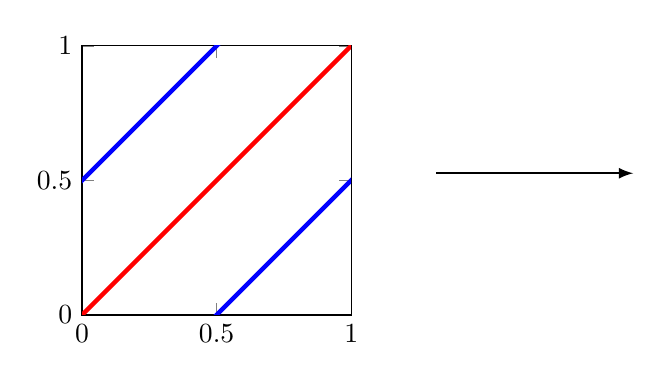
\begin{tikzpicture}
            \begin{axis}[xmax=1,xmin=0, ymin=0,ymax=1, samples=50,width=5cm,height=5cm, xtick={0, 0.5, 1}, ytick={0,0.5,1}]
              \addplot[blue, ultra thick] (x,x+0.5);
              \addplot[red,  ultra thick] (x,x);
              \addplot[blue,  ultra thick] (x,x-0.5);
            \end{axis}
            \draw[thick, -latex] (4.5,1.8) -- (7,1.8);
        \end{tikzpicture}
        \begin{asypicture}{name=torus}
            import graph3;
           
            size(200,0);
            currentprojection=orthographic(4,0,2);
           
            //inner radius
            real R=2;
            //outer radius
            real a=0.75;
           
            //surface:
            triple f(pair t) {
              return ((R+a*cos(t.y))*cos(t.x),(R+a*cos(t.y))*sin(t.x),a*sin(t.y));
            }
           
            real p = 2;
            real q = 2;

            //path:
            real x(real t) {return cos(p*t)*(R + a*cos(q*t));}
            real y(real t) {return sin(p*t)*(R + a*cos(q*t));}
            real z(real t) {return a*sin(q*t);}
           
            real xa(real t) {return -cos(p*t)*(R + a*cos(q*t));}
            real ya(real t) {return sin(p*t)*(R + a*cos(q*t));}
            real za(real t) {return -a*sin(q*t);}

            pen p=blue+opacity(0.33);
            // make surface and path
            surface s=surface(f,(0,0),(2pi,2pi),8,8,Spline);
            path3 q=graph(x,y,z,0,2*pi,operator ..);
            path3 qa = graph(xa,ya,za, 0, 2*pi, operator..);
           
            // draw surface and path
            draw(s,surfacepen=material(diffusepen=white+opacity(0.70), emissivepen=gray));
            real linewidth = 2pt;
            draw(q, p=linewidth + red);
            draw(qa, p=linewidth+blue);
        \end{asypicture}
    \end{center}
    
    So as a topological space, $E\times_{B} E'$ looks like a disjoint union of two circles. As a covering space with the induced map $q : E\times_B E' \to B$, each of these circles wraps twice around $B$, so this is a two sheeted covering of $S^1$, equivalent to the disjoint union of two $z\mapsto z^2$ coverings of the circle.

    \textbf{(c)} Here we can do what we did in (b), but the modulo relation becomes $2\theta_1\equiv 3\theta_2\mod 1$, which looks like:
    \begin{center}
        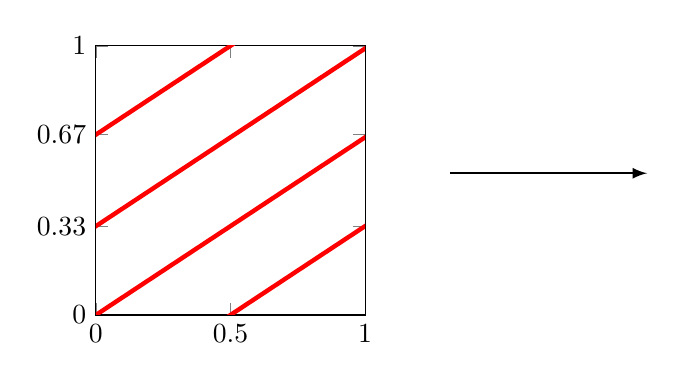
\begin{tikzpicture}
            \begin{axis}[xmax=1,xmin=0, ymin=0,ymax=1, samples=50,width=5cm,height=5cm, xtick={0, 0.5, 1}, ytick={0,0.33, 0.67,1}]
              \addplot[red, ultra thick] (x,0.66*x+0.67);
              \addplot[red,  ultra thick] (x,0.66*x+0.33);
              \addplot[red,  ultra thick] (x,0.66*x);
              \addplot[red,  ultra thick] (x,0.66*x-0.33);
            \end{axis}
            \draw[thick, -latex] (4.5,1.8) -- (7,1.8);
        \end{tikzpicture}
        \begin{asypicture}{name=torus}
            import graph3;
            
            size(200,0);
            currentprojection=orthographic(4,0,2);
            
            //inner radius
            real R=2;
            //outer radius
            real a=0.75;
            
            //surface:
            triple f(pair t) {
              return ((R+a*cos(t.y))*cos(t.x),(R+a*cos(t.y))*sin(t.x),a*sin(t.y));
            }
            
            real p = 2;
            real q = 3;

            //path:
            real x(real t) {return cos(p*t)*(R + a*cos(q*t));}
            real y(real t) {return sin(p*t)*(R + a*cos(q*t));}
            real z(real t) {return a*sin(q*t);}

            pen p=blue+opacity(0.33);
            // make surface and path
            surface s=surface(f,(0,0),(2pi,2pi),8,8,Spline);
            path3 q=graph(x,y,z,0,2*pi,operator ..);
            
            // draw surface and path
            draw(s,surfacepen=material(diffusepen=white+opacity(0.70), emissivepen=gray));
            real linewidth = 2pt;
            draw(q, p=linewidth + red);
        \end{asypicture}
    \end{center}
    This is a connected curve known as a $(2,3)$-torus knot, but as a topological space, $E\times_B E'$ is a circle. The covering map wraps this circle around the base circle $6$ times, so this covering is equivalent to the 6 sheeted covering $z\mapsto z^6$.
\end{solution}

\begin{problem}
    Let $X$ be the figure eight space, with base point $x_0$ where the two circles are glued. Let $a$ and $b$ be the two free generators of $\pi_1(X,x_0)$ corresponding to the loops around each circle. 
    \begin{enumerate}[(a)]
        \item What are the connected degree 2 coverings of $X$ up to equivalence? Draw them! Make sure to label and orient the edges (as in Figure 60.3).
        \item For each covering you drew in (a), give a list of generators for the corresponding subgroup of $\pi_1(X,x_0)$.
    \end{enumerate}
    (Remark: what does this say about index 2 subgroups of the free group on two generators?)
\end{problem}

\begin{solution}
    \textbf{(a)} To classify connected degree $2$ coverings, we start by taking some open neighborhood of the gluing point and looking at its preimage in the covering space. Since the covering is degree $2$, geometrically the preimage looks like two Xs. 

    \begin{center}
        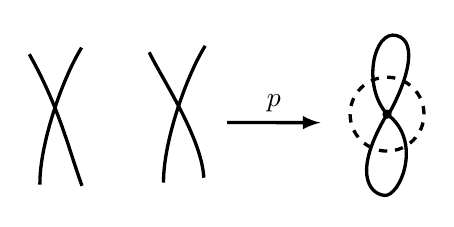
\begin{tikzpicture}[x=0.75pt,y=0.75pt,yscale=-1,xscale=1, very thick]
            %uncomment if require: \path (0,300); %set diagram left start at 0, and has height of 300
            
            %Curve Lines [id:da8856221194251219] 
            \draw    (38.09,209.58) .. controls (37.85,190.87) and (48.55,159.1) .. (58.18,143.62) ;
            %Curve Lines [id:da355859075596322] 
            \draw    (33,146.81) .. controls (47.66,172.9) and (52,192.81) .. (58.38,210.19) ;
            %Curve Lines [id:da406238905716245] 
            \draw    (97.66,208.7) .. controls (97.42,189.99) and (108.11,158.22) .. (117.75,142.74) ;
            %Curve Lines [id:da9006338308522228] 
            \draw    (90.77,145.86) .. controls (97,158.81) and (116,186.81) .. (117.07,206.3) ;
            %Shape: Circle [id:dp598364018945039] 
            \draw  [fill={rgb, 255:red, 0; green, 0; blue, 0 }  ,fill opacity=1 ] (205.35,177.05) .. controls (204.59,177.05) and (203.98,176.44) .. (203.97,175.68) .. controls (203.97,174.92) and (204.58,174.3) .. (205.34,174.3) .. controls (206.1,174.3) and (206.72,174.91) .. (206.72,175.67) .. controls (206.73,176.43) and (206.11,177.05) .. (205.35,177.05) -- cycle ;
            %Curve Lines [id:da39634141071759843] 
            \draw    (205.35,175.68) .. controls (193,161.81) and (199,134.81) .. (210,137.81) .. controls (221,140.81) and (214.53,161.31) .. (205.35,177.05) ;
            %Curve Lines [id:da832615721095836] 
            \draw    (205.35,175.68) .. controls (188.86,203.24) and (196.38,213.89) .. (204,214.81) .. controls (211.62,215.74) and (222.84,188.44) .. (205.35,175.68) -- cycle ;
            
            %Straight Lines [id:da8057379351101164]
            \draw[-latex] (128.29,179.69) -- node[above]{$p$} (173.3,179.78) ;

            %Shape: Circle [id:dp929373118431053] 
            \draw  [dashed] (205.44,193.47) .. controls (195.61,193.52) and (187.6,185.59) .. (187.55,175.77) .. controls (187.5,165.94) and (195.43,157.93) .. (205.26,157.88) .. controls (215.08,157.83) and (223.09,165.76) .. (223.14,175.59) .. controls (223.19,185.41) and (215.26,193.42) .. (205.44,193.47) -- cycle ;
            
        \end{tikzpicture}

    \end{center}
    Then to determine all of the (connected) degree $2$ coverings, it suffices to find all ways to ``connect'' the endpoints in a way which yields a degree $2$ covering. There are exactly three ways:

    \begin{center}
        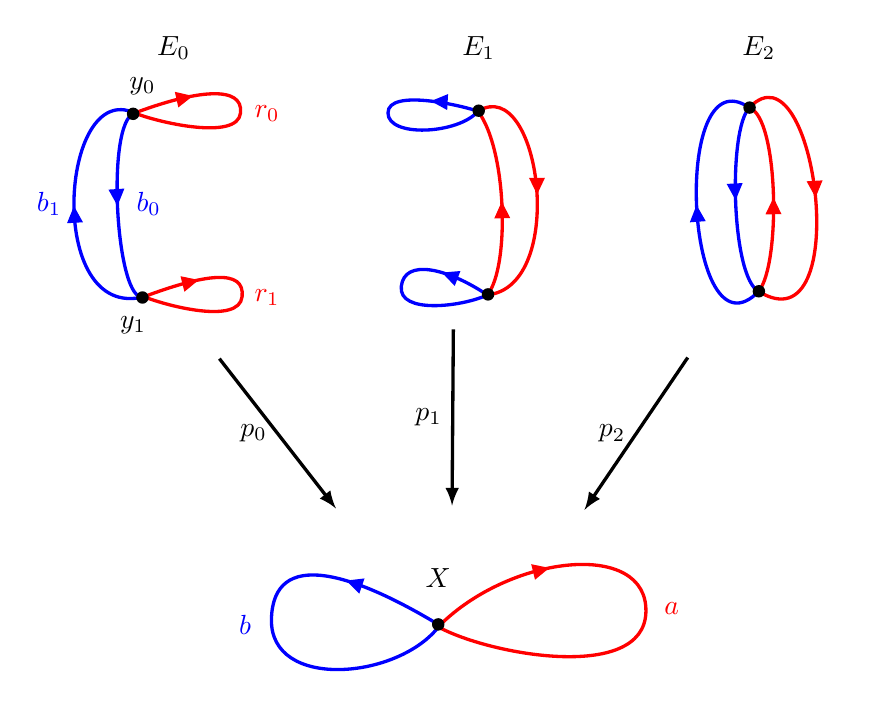
\begin{tikzpicture}[x=0.75pt,y=0.75pt,yscale=-1.5,xscale=1.5, very thick]

            \node[] at (345, 60) {$E_0$};
            \node[] at (443, 60) {$E_1$};
            \node[] at (533, 60) {$E_2$};
            \node[] at (430, 230) {$X$};
            
            %Curve Lines [id:da39634141071759843] 
            \draw[red] (430.48,245.29) .. controls (453.57,222.43) and (497.29,217.86) .. (496.71,241) .. controls (496.14,264.14) and (444.8,254.54) .. (429.11,245.29) ;
            \draw [shift={(465.68,226.86)}, rotate = 166.07] [fill={rgb, 255:red, 255; green, 0; blue, 0 }  ][line width=0.08]  [draw opacity=0] (5.36,-2.57) -- (0,0) -- (5.36,2.57) -- cycle    ;
            %Curve Lines [id:da832615721095836] 
            \draw[blue] (430.48,245.29) .. controls (403,228.66) and (377,220.14) .. (376.43,243.29) .. controls (375.86,266.43) and (417.63,262.71) .. (430.48,245.29) -- cycle ;
            \draw [shift={(400.42,230.93)}, rotate = 18.91] [fill={rgb, 255:red, 0; green, 0; blue, 255 }  ][line width=0.08]  [draw opacity=0] (5.36,-2.57) -- (0,0) -- (5.36,2.57) -- cycle    ;
            
            
            %Curve Lines [id:da6320643571299287] 
            \draw[blue] (335.5,139.75) .. controls (326.5,142.75) and (323,83.25) .. (332.5,80.75) ;
            \draw [shift={(326.98,110.53)}, rotate = 266.32] [fill={rgb, 255:red, 0; green, 0; blue, 255 }  ][line width=0.08]  [draw opacity=0] (5.36,-2.57) -- (0,0) -- (5.36,2.57) -- cycle    ;
            %Curve Lines [id:da14827458293829254] 
            \draw[blue] (335.5,139.75) .. controls (303.57,147.86) and (308.43,69.57) .. (332.5,80.75) ;
            \draw [shift={(313,110.64)}, rotate = 86.48] [fill={rgb, 255:red, 0; green, 0; blue, 255 }  ][line width=0.08]  [draw opacity=0] (5.36,-2.57) -- (0,0) -- (5.36,2.57) -- cycle    ;
            %Curve Lines [id:da20706772794017136] 
            \draw[red] (332.5,80.75) .. controls (352.5,73.25) and (367.5,71.75) .. (366.5,80.75) .. controls (365.5,89.75) and (340,83.75) .. (332.5,80.75) -- cycle ;
            \draw [shift={(351.19,75.27)}, rotate = 167.32] [fill={rgb, 255:red, 255; green, 0; blue, 0 }  ][line width=0.08]  [draw opacity=0] (5.36,-2.57) -- (0,0) -- (5.36,2.57) -- cycle    ;
            %Curve Lines [id:da4034713044779292] 
            \draw[red] (335.5,139.75) .. controls (355.5,132.25) and (368,130.75) .. (367,139.75) .. controls (366,148.75) and (343,142.75) .. (335.5,139.75) -- cycle ;
            \draw [shift={(353.06,134.36)}, rotate = 165.96] [fill={rgb, 255:red, 255; green, 0; blue, 0 }  ][line width=0.08]  [draw opacity=0] (5.36,-2.57) -- (0,0) -- (5.36,2.57) -- cycle    ;
            
            
            %Curve Lines [id:da14638425639362018] 
            \draw[red] (445.79,139.18) .. controls (453,130.14) and (452.14,92.71) .. (442.79,80.18) ;
            \draw [shift={(450.41,109.18)}, rotate = 88.39] [fill={rgb, 255:red, 255; green, 0; blue, 0 }  ][line width=0.08]  [draw opacity=0] (5.36,-2.57) -- (0,0) -- (5.36,2.57) -- cycle    ;
            %Curve Lines [id:da16977100749734508] 
            \draw[red] (445.79,139.18) .. controls (471.86,136.43) and (462.71,67.86) .. (442.79,80.18) ;
            \draw [shift={(461.75,106.91)}, rotate = 269.68] [fill={rgb, 255:red, 255; green, 0; blue, 0 }  ][line width=0.08]  [draw opacity=0] (5.36,-2.57) -- (0,0) -- (5.36,2.57) -- cycle    ;
            %Curve Lines [id:da6792506340753368] 
            \draw[blue] (442.79,80.18) .. controls (436.43,87.57) and (413.86,88.71) .. (413.86,80.71) .. controls (413.86,72.71) and (437.86,78.43) .. (442.79,80.18) -- cycle ;
            \draw [shift={(427.67,76.92)}, rotate = 3.25] [fill={rgb, 255:red, 0; green, 0; blue, 255 }  ][line width=0.08]  [draw opacity=0] (5.36,-2.57) -- (0,0) -- (5.36,2.57) -- cycle    ;
            %Curve Lines [id:da5134456185117895] 
            \draw[blue] (445.79,139.18) .. controls (432.71,130.43) and (419.14,127.43) .. (418.14,136.43) .. controls (417.14,145.43) and (437.57,143) .. (445.79,139.18) -- cycle ;
            \draw [shift={(431.21,131.99)}, rotate = 20.83] [fill={rgb, 255:red, 0; green, 0; blue, 255 }  ][line width=0.08]  [draw opacity=0] (5.36,-2.57) -- (0,0) -- (5.36,2.57) -- cycle    ;

            
            %Curve Lines [id:da1416284010003046] 
            \draw[red] (532.93,138.04) .. controls (540.14,129) and (539.29,82.14) .. (529.93,79.04) ;
            \draw [shift={(537.69,107.9)}, rotate = 89.97] [fill={rgb, 255:red, 255; green, 0; blue, 0 }  ][line width=0.08]  [draw opacity=0] (5.36,-2.57) -- (0,0) -- (5.36,2.57) -- cycle    ;
            %Curve Lines [id:da4356562252432308] 
            \draw[red] (532.93,138.04) .. controls (564.14,157.29) and (551.29,56.43) .. (529.93,79.04) ;
            \draw [shift={(551.2,107.88)}, rotate = 266.62] [fill={rgb, 255:red, 255; green, 0; blue, 0 }  ][line width=0.08]  [draw opacity=0] (5.36,-2.57) -- (0,0) -- (5.36,2.57) -- cycle    ;
            %Curve Lines [id:da8498955808251791] 
            \draw[blue] (532.93,138.04) .. controls (509.29,162.14) and (504.43,61.29) .. (529.93,79.04) ;
            \draw [shift={(512.97,110.32)}, rotate = 85.76] [fill={rgb, 255:red, 0; green, 0; blue, 255 }  ][line width=0.08]  [draw opacity=0] (5.36,-2.57) -- (0,0) -- (5.36,2.57) -- cycle    ;
            %Curve Lines [id:da759972606551601] 
            \draw[blue] (532.93,138.04) .. controls (524.14,133.57) and (523,86.14) .. (529.93,79.04) ;
            \draw [shift={(525.51,108.73)}, rotate = 266.82] [fill={rgb, 255:red, 0; green, 0; blue, 255 }  ][line width=0.08]  [draw opacity=0] (5.36,-2.57) -- (0,0) -- (5.36,2.57) -- cycle    ;
            
            
            \fill[] (533, 138) circle (2);
            \fill[] (530, 79) circle (2);
            
            \fill[] (446, 139) circle (2);
            \fill[] (443, 80) circle (2);
            
            \fill[] (335, 140) circle (2);
            \fill[] (332, 81) circle (2);
            
            \node[red] at (375,140) {$r_1$};
            \node[red] at (375,81) {$r_0$};
            \node[blue] at (337,110) {$b_0$};
            \node[blue] at (305,110) {$b_1$};
            
            \node[] at (335,72) {$y_0$};
            \node[] at (332,149) {$y_1$};
            
            \node[red] at (505,240) {$a$};
            \node[blue] at (368,245) {$b$};

            \fill[] (430, 245) circle (2);

            \draw[-latex] (359.71,159.64) -- node[left]{$p_0$} (397.16,207.77);
            \draw[-latex] (434.86,150.21) -- node[left]{$p_1$} (434.45,206.86);
            \draw[-latex] (510.14,159.29) -- node[left]{$p_2$} (476.97,208.23);
        \end{tikzpicture}
    \end{center}
    
    The spaces $E_0, E_1, E_2$ have natural covering maps $p_0, p_1, p_2$ as shown in the diagram. For example the map $p_0 : E_0 \to X$ maps the red loops in $E_0$ homeomorphically onto the red loop in $X$, and maps each blue path in $E_0$ onto the blue loop in $X$. It's clear that these are all degree $2$ coverings of $X$.

    \textbf{(b)} We'll calculate the corresponding subgroup of $F_2$ for $E_0$ explicitly, the rest follow similarly. Applying the Seifert Van Kampen theorem to $E_0$, spitting it along some small open neighborhood or $y_0$, we get that $\pi_1(E_0, y_0)$ is generated by the loops $r_0$, $b_0*r_1*b_1$, and $b_0*b_1$. Letting $a$ be the loop in $X$ going around the red loop clockwise and $b$ be the loop in $X$ going counterclockwise around the blue loop. These generate $\pi_1(X,x_0)\cong F_2$. The induced subgroup of $F_2$ by $E_0$ is then generated by the images of the generators of $\pi_1(E_0,y_0)$ under the covering map $p_0$. Note that
    \[
        \begin{aligned}
            p_0\circ r_0 &= a\\
            p_0\circ (b_0*r_1*b_1) &= bab\\
            p_0\circ (b_0*b_1) &= b^2
        \end{aligned}
    \]
    so $(p_0)_*(\pi_1(E_0,y_0))=\big\langle a,bab, b^2 \big\rangle$. Similarly we have $(p_1)_*(\pi_1(E_1,y_0))=\big\langle a^2, aba, b \big\rangle$ and $(p_2)_*(\pi_1(E_2, y_0))=\big\langle a^2,ab, ab^{-1} \big\rangle$. By the classification of covering spaces, these are all of the index two subgroups of $F_2$. 
\end{solution}

\begin{problem}
    What is the fundamental group of a torus with one point removed?  With two points removed? Can you come up with an example of a degree 2 covering map between these two spaces?
\end{problem}

\begin{solution}
    Recall from the previous problem set that we can find a deformation retraction of $T-\{p\}$ onto a wedge of two circles $S^1\vee S^1$ and so $\pi_1(T-\{p\})$ is isomorphic to $F_2$, the free group on two generators. Similarly, we can find a deformation retraction of $T-\{p,q\}$ onto a wedge of three circles $S^1\vee S^1\vee S^1$ and so $\pi_1(T-\{p,q\})$ is isomorphic to $F_3$, the free group on three generators. In light of the counterintuitive group embedding $F_3\to F_2$ from 55a, we'll try to construct a two sheeted covering map from $T-\{p,q\}$ to $T-\{p\}$. 
    
    Consider the two sheeted covering $f : S^1 \to S^1$ given by $z\mapsto z^2$ where $z\in S^1$ is considered as a complex number. This defines a two sheeted covering $g=f\times \id_{S^1} : T \to T$. Then if we pick some point $p\in T$, and let $\{q_1,q_2\}=g^{-1}(p)$ we have an induced two sheeted covering map $\restr{g}{T-\{q_1,q_2\}} : T-\{q_1,q_2\} \to T-\{p\}$. This induces an injective group homomorphism $g_* : F_3 \to F_2$.
\end{solution}


\end{document}